\documentclass[tikz]{standalone}
\usetikzlibrary{spy,shapes,shadows,calc,pgfplots.groupplots}
\usepackage{amsmath}
\usepackage{physics} 
\usepackage{pgfplots}
\pgfplotsset{compat=1.3}
\usepackage{amsmath}
\DeclareFontFamily{OT1}{pzc}{}
\DeclareFontShape{OT1}{pzc}{m}{it}{<-> s * [1.10] pzcmi7t}{}
\DeclareMathAlphabet{\mathpzc}{OT1}{pzc}{m}{it}
\newcommand{\ddtn}{\operatorname{dtn}}

\pgfplotsset{
  legend style = {font=\small}
}

\begin{document}
\begin{tikzpicture}[scale = 0.8]

%\begin{axis}[
\begin{scope}[ ]
\node (diffB) at (0,2.5) {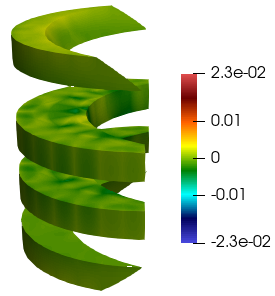
\includegraphics[scale =.35]{diff-B.png}};
\draw[] (0,-0.5)   node[draw, fill=white, minimum size=0.5mm]{ $u - \underline{u}_1$ in $B$ };
\end{scope}
\begin{scope}[xshift=3cm ]
\begin{groupplot}[
    group style={
        %group name=dtn,
        group size=1 by 1,
        %xticklabels at=edge bottom,
        horizontal sep=25pt,
        vertical sep=40pt,
   },
   %name = dtnplot,
   height = 6.5cm,
   width = 8.5cm,
   every axis plot/.append style={thick},
   axis y line*=left,
   legend pos = south east,
   %xmin = 0,
   %xmax = 11000,
   %ymin = -20,
   %ymax = 20,
   %restrict y to domain=-1e2:1e2,
   %label style={at={(axis description cs:0.5,-0.08)},anchor=north},
   %every x tick scale label/.style={at={(xticklabel cs:0.925)},anchor=south west},
   %x label style={at={(axis description cs:0.975,0.085)},anchor=east},
   %xlabel= { $\lambda$},
    legend style = { column sep = 10pt, legend columns = 2, legend to name = grouplegend,},
   ]
    
    \nextgroupplot[ 
    ymode=log,
    xmode=log,
    %xmin=0,xmax=1.6e4,
    %xtick={25, 125, 250, 500, 800, 1000},
    %axis x line*=middle,
    %axis y line=middle, 
    ymax = 2e-0,
    %ymax = 350,
    %width=9cm,
    %restrict y to domain=-4e2:4e2,
    %xtick={0,2e3,4e3,6e3,8e3,10e3,12e3,14e3},
    xlabel= { $ (2T/N) \sim h$},
    %legend pos = south west,
    legend style = { column sep = 10pt, legend columns = 3, legend to name = grouplegend,},
    x label style={at={(axis description cs:0.9,0.06)},anchor=east},
    title = {  $\norm{ u - \underline{u}_1 }_{L^2(Q \setminus B )}$ },
    %title = {   $ $  },
    legend style={at={(0.5,-0.1)},anchor=north},
	]

    \addplot[red,very thick,mark=*] 
    	table[x=deltat,y=L2-err-Bcompl] {../data/Cylinder--q1-qstar1-k1-kstar1-msol2.dat}; \addlegendentry{$ q = 1 $ }%
    \addplot[blue,very thick,mark=triangle]  
	table[x=deltat,y=L2-err-Bcompl] {../data/Cylinder--q2-qstar0-k2-kstar1-msol2.dat}; \addlegendentry{$ q = 2$}%
    %\addplot[green!70!black,very thick,mark=diamond] 
    %	table[x=deltat,y=L2-err-Bcompl] {../data/Cylinder--q3-qstar0-k3-kstar1-msol2.dat};  \addlegendentry{$ q = 3$ }%
    
    \addplot[lightgray,dashed,line width=3pt ,forget plot] 
	table[mark=none,x=deltat,y expr ={ 0.45/ abs(ln(  (\thisrowno{0} ) ) )    }] {../data/Cylinder--q1-qstar1-k1-kstar1-msol2.dat};
	%table[mark=none,x=deltat,y expr ={ 1.0/ abs(ln(  (\thisrowno{0}) ))  }] {../data/Cylinder--q1-qstar1-k1-kstar1.dat};
	%table[mark=none,x=deltat,y expr ={ 0.4/ abs(ln( abs( ln( (\thisrowno{0}) ))))  }] {../data/Cylinder--q1-qstar1-k1-kstar1.dat};
    \addplot[lightgray,dashdotted,ultra thick,forget plot] 
    	table[mark=none,x=deltat,y expr ={0.035/ abs(ln(  (\thisrowno{0} ) ) )^2   } ] {../data/Cylinder--q2-qstar0-k2-kstar1-msol2.dat};
    %\addplot[lightgray,dotted,ultra thick,forget plot] 
    %	table[mark=none,x=deltat,y expr ={0.005/ abs(ln(  (\thisrowno{0} ) ) )   } ] {../data/Cylinder--q3-qstar0-k3-kstar1-msol2.dat};

    \draw[] (axis cs:0.09,3.5e-1)   node[rotate=5, minimum size=0.5mm]{ $ \mathcal{O}( \vert \log(h) \vert^{-1}  )  $   };
    \draw[] (axis cs:0.08,9.5e-3)   node[rotate=15, minimum size=0.5mm]{ $ \mathcal{O}( \vert \log(h) \vert^{-2}  ) $   };
    %\draw[] (axis cs:0.3,2.5e-3)   node[rotate=20, minimum size=0.5mm]{ $ \mathcal{O}( \vert \log(h) \vert^{-1}  ) $   };
 
    \end{groupplot}
    \node at ($(group c1r1) + (-0.0cm,-3.45cm)$) {\ref{grouplegend}}; 
 \end{scope}

\begin{scope}[xshift=13cm ]
\node (diffB) at (0,2.5) {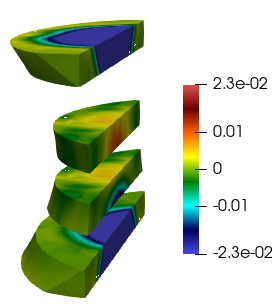
\includegraphics[scale =.35]{diff-B-compl.png}};
\draw[] (0,-0.75)   node[draw, fill=white, minimum size=0.5mm]{ $u - \underline{u}_1$ in $Q \setminus B$ };
\end{scope}

\end{tikzpicture}
\end{document}





